\section{Examples of Tangible User Interfaces}
There is a wide variety of Tangible User Interfaces (TUIs). Possible applications for TUIs are literally endless. Many systems of TUIs have been explored and published in the past, but still a lot of new a ideas are coming up and new applications for TUIs are going to be explored. In this section, we will give examine some examples of TUIs and give an overview of different domains where TUIs have been successfully deployed.

\subsection{Table-top environments}
Many TUIs rely on table-top environments as their interaction technique. In these environments, a IR camera is set underneath the table-top to track fiducial markers placed onto the table. The camera can also track touch interactions of users. Marker and touch-based interactions are used as user input to the TUI system. The system responds to the user interactions by projecting visual feedback onto the table-top.

\subsubsection{reacTable}
The reactAble, presented by \cite{jorda07}, is a musical instrument based on a table-top TUI. Fiducial Markers represent musical objects, which generate sound according to their relation to each other. The markers are tracked by an IR camera. According to their attached symbol, each object has a dedicated function. The objects can be categorized in six different functional groups: audio generators, audio filters, controllers, control filters, mixers and global objects. \shortcite{jorda07}

ReacTIVision, the computer vision system behind reactAble, tracks the fiducial markers and sends the output data to an audio synthesizer. The waveforms generated by the synthesizer, as well as the data from the ReacTIVision tracker are sent to a visual synthesizer. The visual synthesizer projects visual feedback back onto the table-top. The audio lines that connect objects show the real resulting waveforms. Visual feedback is also used to monitor the objects state and internal parameters. Fingers can be used to either modify the objects parameters, or to cut (i.e. mute) audio connections between objects. \shortcite{jorda07}

\begin{figure}
\centering
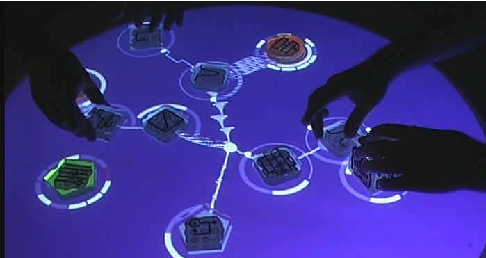
\includegraphics[width=0.45\textwidth]{figures/reactable.pdf}
\caption{The reacTable in action (compare \shortcite{jorda07})}
\label{fig:reactable}
\end{figure}
%TODO: reference figure!!

Modular synthesis is used for the sound generation process. Modular synthesis is based on the interconnection of sound generators and sound processor units. In reactAble, automatic connections between objects are made depending on the type of objects involved and the proximity between them. By moving objects around and bringing them into relation to each other, performers construct and play instruments at the same time. reactAble is also a collaborative tool for interactive live music. Because of the rather big size of the table-top, multiple artists can perform together on a single reacTable. \shortcite{jorda07}

\subsubsection{TARboard}
TARBoard is a tangible augmented reality system designed for table-top game environment. The purpose of TARboard is is to let users enjoy games in a more interactive and intuitive way and to make games more realistic and immersive. \shortcite{lee05}

Markers are attached to objects or cards used in a game. Similar to reactAble, these markers are tracked on a table-top environment by a camera underneath it. The augmenting camera is placed above the table-top. It provides the video stream for augmenting a game with virtual objects. \shortcite{lee05}

\cite{lee05} implemented a card game as a prototype for TARboard. Each player has cards which represent mystic creatures. The marker on the bottom of each card is tracked by the tracking camera. When the players flip a card and place it near the battle zone, the creatures get augmented on the battle zone and fight against each other.

\subsection{Urban planning workbenches}
In urban planning, designers usually employ three forms of representation: Two-dimensional drawings on sheets of papers, three-dimensional physical models and computer models, which can be two and three-dimensional. Each of these representations are created and displayed independently. Urban planning workbenches try to bridge the gap between these forms of representation, by simultaneously layering 2D drawings, 3D physical models, and digital simulation over each other. 
First, the 2D drawings and sketches are laid out on a table. Next, the 3D models are placed on top of the drawings. Finally, video projectors project digital simulations onto the surface. Video cameras capture the activity on the table and adjust the dynamic representation according to the position of the drawings and models with optical tags. \cite{ishii02}

\subsubsection{Urp}


\subsubsection{The Luminous Table}
